\documentclass[12pt,a4paper]{article}

%------------------------------------------------
% Packages
%------------------------------------------------
\usepackage[T1]{fontenc}
\usepackage{lmodern}
\usepackage{graphicx}
\usepackage{amsmath,amssymb}
\usepackage{siunitx}
\usepackage{geometry}
\usepackage{fancyhdr}
\usepackage{booktabs}
\usepackage{caption}
\usepackage{float}
\usepackage{subcaption}
\usepackage{array}
\usepackage[dvipsnames]{xcolor}
\usepackage{setspace}
\usepackage[hidelinks]{hyperref}
\usepackage[backend=biber,style=numeric]{biblatex}

\addbibresource{references.bib}

%------------------------------------------------
% Page layout
%------------------------------------------------
\geometry{
    top=1in,
    bottom=1.2in,
    left=1in,
    right=1in
}

\setlength{\headheight}{15pt}
\setlength{\parskip}{0.4em}
\setlength{\parindent}{0pt}

\pagestyle{fancy}
\fancyhf{}
\fancyhead[L]{Ian Cullinane}
\fancyhead[R]{Planck’s Constant}
\fancyfoot[C]{\thepage}

\sisetup{
    inter-unit-product = \cdot,
    uncertainty-mode = separate,
    per-mode = symbol
}

%------------------------------------------------
% Title
%------------------------------------------------
\title{
    \Large\textbf{Investigating the Photoelectric Effect: An Experimental Determination of Planck’s Constant.}\\[0.5em]
    \large PY2107 -- Experiment 7
}

\author{
    Ian Cullinane -- \textit{125413342}\\[0.5em]
    Lab Partner: Fionn Lichtsinn Doyle\\[0.5em]
    Demonstrators: Jonathan and Olivia
}

\date{7th September 2026}

\begin{document}

\maketitle
\thispagestyle{empty}

\newpage
\tableofcontents
\newpage

%================================================
\section{Abstract}
%================================================

The photoelectric effect was investigated to estimate Planck's constant and the effective work function of a caesium-coated cathode. Light-emitting diodes (LEDs) of different wavelengths illuminated a vacuum photocell, and their stopping potentials were measured. LED wavelengths were determined independently from diffraction-grating maxima. A five-point fit of stopping potential against reciprocal wavelength gave \(h_{\mathrm{exp}}=(6.4\pm0.4)\times10^{-34}\,\mathrm{J\,s}\), 4.2\% below the accepted value, and an effective work function of \((1.7\pm0.1)\,\mathrm{eV}\). These uncertainties combine diffraction-fit variation with propagated position and distance errors while treating the voltage readings as exact. Stopping potential was also measured over a range of intensities for three LEDs. Its broadly intensity-independent behaviour is consistent with the prediction that photon frequency, rather than intensity, sets the maximum photoelectron energy, although anomalous low-intensity data limit this test. A separate photocurrent--voltage sweep showed a saturating trend but had an uncorrected current offset. Overall, the measurements provide quantitative, but uncertainty-limited, evidence consistent with Einstein's light-quantum relation; they do not by themselves constitute a definitive proof of photon quantisation.

\newpage

%================================================
\section{Theory}
%================================================

The photoelectric effect is the emission of electrons from a material when electromagnetic radiation of sufficiently high frequency is incident upon its surface. In 1905, Einstein proposed that light transfers energy in discrete quanta, each with energy \(hf\), and used this idea to explain the frequency dependence of photoelectron energy \cite{einstein1905}. This experiment tests that specific prediction by measuring the stopping potential at several light frequencies. Agreement with the predicted linear relation is evidence consistent with the light-quantum model, while the finite data set and measurement uncertainties mean that it should not be described as a stand-alone proof of quantisation. Millikan's later precision measurements provided a historically important quantitative test of Einstein's equation \cite{millikan1916}.

\subsection{Einstein's Photoelectric Equation}

In Einstein's light-quantum model, each photon carries energy proportional to the frequency of the radiation \cite{einstein1905}:

\begin{equation}
    E_{\gamma} = hf,
    \label{eq:photon_energy}
\end{equation}

where \(E_{\gamma}\) is the photon energy, \(h\) is Planck's constant, and \(f\) is the frequency of the incident radiation.

When a photon interacts with an electron in the metal, its energy is transferred to the electron. A minimum energy, known as the work function \(\phi\), is required for an electron to escape from the metal surface. Any energy remaining after overcoming the work function is converted into the kinetic energy of the emitted electron. Conservation of energy therefore gives Einstein's photoelectric equation \cite{einstein1905}:

\begin{equation}
    K_{\max} = hf - \phi,
    \label{eq:einstein}
\end{equation}

where \(K_{\max}\) is the maximum kinetic energy of the emitted photoelectrons.

The work function depends on the material and its surface properties. In the single-photon regime considered here, if the photon energy is less than the work function, photoemission does not occur merely by increasing the intensity. The minimum frequency required to produce photoemission is called the threshold frequency, \(f_0\). At this frequency, the emitted electrons have zero maximum kinetic energy, so

\begin{equation}
    \phi = hf_0.
    \label{eq:threshold}
\end{equation}

Since the frequency and wavelength of electromagnetic radiation are related by \(c=f\lambda\), where \(c\) is the speed of light in vacuum, the photon energy can also be expressed as

\begin{equation}
    E_{\gamma} = \frac{hc}{\lambda}.
    \label{eq:wavelength_energy}
\end{equation}

Substituting this expression into Equation~\ref{eq:einstein} gives

\begin{equation}
    K_{\max} = \frac{hc}{\lambda} - \phi.
    \label{eq:einstein_wavelength}
\end{equation}

\subsection{Stopping Potential}

In the experimental apparatus, the photocathode and anode are enclosed in an evacuated tube. When the cathode is illuminated, photoelectrons are emitted and collected by the anode, producing a measurable electric current.

A reverse potential difference is applied between the electrodes to oppose the motion of the emitted electrons. As the magnitude of this reverse potential increases, fewer electrons have sufficient kinetic energy to reach the anode. The stopping potential, \(V_{\max}\), is the magnitude of the reverse potential required to reduce the photocurrent to zero.

The electric potential energy associated with an electron passing through a potential difference of magnitude \(V_{\max}\) is \(eV_{\max}\), where \(e\) is the elementary charge. At the stopping potential, this energy equals the maximum kinetic energy of the emitted photoelectrons:

\begin{equation}
    K_{\max} = eV_{\max}.
    \label{eq:stopping}
\end{equation}

Combining Equations~\ref{eq:einstein_wavelength} and \ref{eq:stopping} gives

\begin{equation}
    eV_{\max} = \frac{hc}{\lambda} - \phi.
\end{equation}

Rearranging yields the relationship between stopping potential and wavelength:

\begin{equation}
    V_{\max} = \frac{hc}{e}\frac{1}{\lambda}
    - \frac{\phi}{e}.
    \label{eq:stopping_wavelength}
\end{equation}

Alternatively, expressing the work function in terms of the threshold wavelength \(\lambda_0\), for which \(\phi=hc/\lambda_0\), gives

\begin{equation}
    V_{\max} = \frac{hc}{e}
    \left(\frac{1}{\lambda}-\frac{1}{\lambda_0}\right).
    \label{eq:threshold_wavelength}
\end{equation}

Equation~\ref{eq:stopping_wavelength} has the form of a straight-line equation, \(y=mx+b\), where \(V_{\max}\) is plotted against \(1/\lambda\). The gradient \(m\) and vertical intercept \(b\) are

\begin{equation}
    m = \frac{hc}{e},
    \qquad
    b = -\frac{\phi}{e}.
    \label{eq:gradient_intercept}
\end{equation}

Consequently, Planck's constant can be determined from the gradient:

\begin{equation}
    h = \frac{me}{c},
    \label{eq:planck}
\end{equation}

and the work function of the cathode can be determined from the intercept:

\begin{equation}
    \phi = -eb.
    \label{eq:work_function}
\end{equation}

If the work function is expressed in electronvolts, the numerical value of the work function in eV is equal to the magnitude of the intercept in volts. The accepted value of Planck's constant is \(6.62607015\times10^{-34}\,\mathrm{J\,s}\), exact in the SI \cite{nistconstants}.

\subsection{Wavelength Calibration Using a Diffraction Grating}

The wavelengths of the LEDs are determined independently using a diffraction grating. A diffraction grating consists of a large number of equally spaced slits, which produce maxima at angles determined by constructive interference.

The condition for a diffraction maximum is \cite{py2107}

\begin{equation}
    d\sin\theta = n\lambda,
    \label{eq:grating}
\end{equation}

where \(d\) is the separation between adjacent grating lines, \(\theta\) is the diffraction angle measured relative to the straight-through direction, \(n\) is the diffraction order, and \(\lambda\) is the wavelength of the light.

If the grating has \(N\) lines per millimetre, the grating spacing in SI units is

\begin{equation}
    d = \frac{10^{-3}}{N}\,\mathrm{m}.
    \label{eq:grating_spacing}
\end{equation}

For a measured diffraction order \(n\), the wavelength is

\begin{equation}
    \lambda = \frac{d\sin\theta}{n}.
    \label{eq:wavelength}
\end{equation}

If a maximum of order \(n\) is displaced by a distance \(x\) from the central maximum and the perpendicular distance between the grating and the measurement scale is \(L\), the diffraction angle can be calculated geometrically:

\begin{equation}
    \tan\theta = \frac{x}{L},
\end{equation}

giving

\begin{equation}
    \theta = \tan^{-1}\left(\frac{x}{L}\right).
    \label{eq:angle}
\end{equation}

Combining these equations gives the wavelength in terms of the measured distances and diffraction order:

\begin{equation}
    \lambda =
    \frac{d}{n}\sin\left[\tan^{-1}\left(\frac{x}{L}\right)\right].
    \label{eq:measured_wavelength}
\end{equation}

The uncertainties in \(x\), \(L\), and the grating spacing contribute to the uncertainty in the calculated wavelength. These uncertainties must be considered when fitting the stopping-potential data, since the wavelength measurements determine the horizontal-axis values in the linear plot.

\subsection{Effect of Light Intensity}

The photoelectric effect also provides a distinction between the effects of light intensity and frequency. For light with a frequency above the threshold frequency, increasing the intensity increases the number of incident photons per unit time. This generally increases the number of emitted photoelectrons per unit time and therefore increases the photocurrent.

However, the energy of an individual photon depends on its frequency rather than its intensity. Consequently, at a fixed frequency, increasing the intensity should not increase the maximum kinetic energy of the emitted electrons. Since the stopping potential is related to the maximum kinetic energy by Equation~\ref{eq:stopping}, the stopping potential is expected to remain approximately constant as the intensity changes.

This intensity-independence is part of the photoelectric behaviour reported by Lenard and explained by Einstein's light-quantum model \cite{lenard1902,einstein1905}. Here, measurements at different LED intensity settings test whether the stopping potential remains approximately constant at fixed frequency.

\subsection{Photocurrent--Voltage Characteristic}

The photocurrent also depends on the potential difference between the photocathode and collecting electrode. A retarding potential opposes the motion of emitted electrons, reducing the fraction that reach the collector. At the stopping potential, even the most energetic photoelectrons are prevented from reaching it, and the photocurrent falls to zero. With a collecting potential, more emitted electrons are collected; once all available photoelectrons are collected, the current approaches a saturation value. Thus, the idealised characteristic rises from zero photocurrent at a negative stopping potential and levels off at positive collecting potentials.

The saturation current depends on the rate of photoelectron emission and therefore generally increases with light intensity. By contrast, the stopping potential is set by the maximum photoelectron kinetic energy and depends on the light frequency, not its intensity. The measured current zero must be distinguished from the photocurrent zero: any dark current or instrument offset shifts the measured curve vertically and makes its raw zero crossing unsuitable as a stopping-potential measurement until the offset is removed.

\subsection{Determination of Uncertainties}

The uncertainty in the calculated Planck constant depends on the uncertainty in the fitted gradient. If the fitted gradient is \(m\pm\Delta m\), then, treating the elementary charge and the speed of light as exact for the purposes of this experiment, the uncertainty in Planck's constant is

\begin{equation}
    \Delta h = \frac{e}{c}\Delta m.
    \label{eq:uncertainty_h}
\end{equation}

Similarly, if the fitted intercept is \(b\pm\Delta b\), the uncertainty in the work function is

\begin{equation}
    \Delta\phi = e\Delta b.
    \label{eq:uncertainty_phi}
\end{equation}

These expressions assume that the uncertainties are obtained from the linear regression and that correlations between the fitted gradient and intercept can be neglected for the individual uncertainty estimates. If the uncertainties are correlated, their covariance should be considered when calculating derived quantities.

The experimental values can be compared with accepted values using the percentage difference:

\begin{equation}
    \text{Percentage difference}
    = \frac{|q_{\mathrm{exp}}-q_{\mathrm{ref}}|}
    {|q_{\mathrm{ref}}|}\times100\%,
    \label{eq:percentage_difference}
\end{equation}

where \(q_{\mathrm{exp}}\) is the experimentally determined quantity and \(q_{\mathrm{ref}}\) is its accepted reference value. Agreement should also be assessed by comparing the difference between the experimental and reference values with the experimental uncertainty.

\newpage

%================================================
\section{Experimental Procedure}
%================================================

Following the course laboratory handout \cite{py2107}, the experiment comprised wavelength calibration, stopping-potential measurements, intensity-dependence measurements, and a separate photocurrent--voltage sweep.

\subsection{Wavelength Calibration of the LEDs}

The wavelengths of the LEDs were determined using a diffraction grating, a slit, and a metre stick. The experimental arrangement is shown in Figure~\ref{fig:apparatus}.

The number of lines per millimetre on the diffraction grating was recorded and used to calculate the grating spacing, \(d\). Each LED was positioned to illuminate the slit, and visible diffraction maxima were identified. The displacement, \(x\), of each maximum from the central, straight-through position was measured using the metre stick. The distance, \(L\), between the grating and the measurement scale was also recorded.

The diffraction angle was calculated using

\begin{equation}
    \theta = \tan^{-1}\left(\frac{x}{L}\right),
\end{equation}

and the wavelength of each LED was determined from the diffraction grating equation,

\begin{equation}
    \lambda = \frac{d\sin\theta}{n},
\end{equation}

using the measured diffraction order \(n\). First- and second-order maxima were recorded where visible, and the calculation was repeated for each LED and each recorded maximum. Numerical uncertainties for the measured distances were not retained in the report, so no numerical wavelength uncertainties can be reported.

\subsection{Measurement of the Stopping Potential}

The second stage of the experiment used a photocell containing a caesium-coated cathode and an anode enclosed in an evacuated tube. The apparatus included a voltmeter to measure the potential difference, a nanoammeter to measure the photocurrent, and a power supply to adjust the reverse potential.

Each LED was inserted into the collector tube to illuminate the photocathode. The LED intensity was set to approximately \(75\%\). The fine adjustment control for the back-emf was initially placed near its central position, and the apparatus was allowed to stabilise for several minutes.

The coarse adjustment control was used to bring the photocurrent approximately to zero. The fine adjustment control was then used to obtain a more accurate zero-current reading. The corresponding stopping potential, \(V_{\max}\), was recorded. This procedure was repeated for each LED, keeping the intensity setting approximately constant.

The independently measured wavelengths from the first stage were used in the subsequent analysis. The stopping potentials were plotted against the reciprocal wavelengths, \(1/\lambda\), to investigate the linear relationship predicted by Einstein's photoelectric equation. The gradient and vertical intercept of the best-fit line were used to determine Planck's constant and the work function of the cathode, respectively.

\subsection{Investigation of Light Intensity}

For the intensity series, the intensity of each of three LEDs was varied over the recorded settings. At each setting, the photocurrent was brought to the instrument-indicated zero using the adjustment controls, and the stopping-potential readings were recorded. The other experimental conditions were kept as consistent as possible.

The measured stopping potentials were plotted against the corresponding LED intensity settings to investigate the relationship between light intensity and the maximum kinetic energy of the emitted photoelectrons. The observed trend was compared with Einstein's prediction, supported by Lenard's observations, that the maximum kinetic energy depends on frequency rather than intensity \cite{einstein1905,lenard1902}.

At the end of the experiment, the empty protective sleeve was slid back over the collector tube to protect the photocell.

\subsection{Photocurrent--Voltage Measurement}

A separate photocurrent--voltage characteristic was recorded by varying the electrode voltage and measuring the current. The report does not specify the illumination conditions for this sweep.
For the plot and sigmoid fit, both recorded channels were sign-reversed (\(V=-V_{\mathrm{recorded}}\), \(I=-I_{\mathrm{recorded}}\)); the data table retains the recorded signs.

\begin{figure}[H]
    \centering
    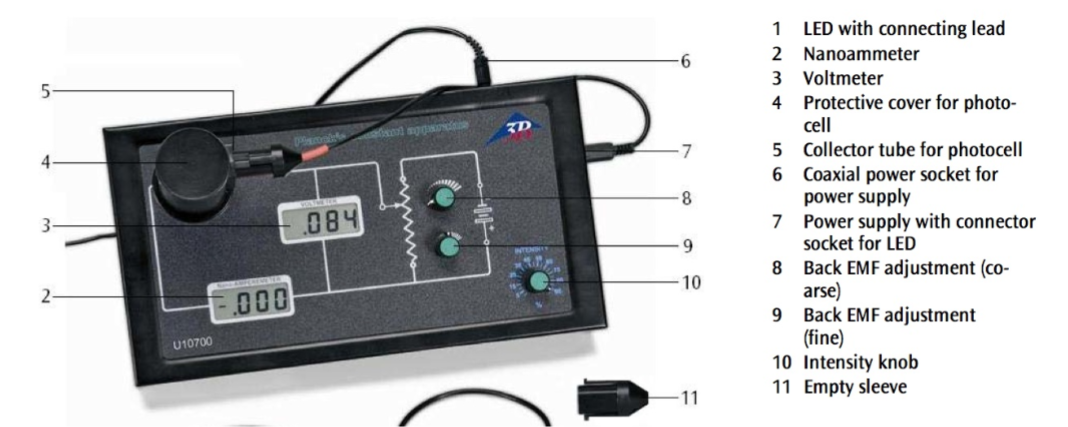
\includegraphics[width=0.8\textwidth]{images/Apparatus.png}
    \caption{Experimental apparatus used to investigate the
    photoelectric effect.}
    \label{fig:apparatus}
\end{figure}

\newpage

%================================================
\section{Analysis}
%================================================
\subsection{Wavelength Calibration}

The wavelengths of the LEDs were determined using a diffraction grating with a spacing of approximately \(1.667\times10^{-6}\,\mathrm{m}\), corresponding to 600 lines per millimetre. The wavelength was calculated from the diffraction equation,

\begin{equation}
    \lambda = \frac{d\sin\theta}{n},
\end{equation}

where \(d\) is the grating spacing, \(\theta\) is the diffraction angle, and \(n\) is the diffraction order.

The measured wavelengths ranged from approximately \(459\) to \(634\,\mathrm{nm}\). The corresponding frequencies were calculated from \(f=c/\lambda\).

The wavelength measurements were subsequently used to determine the frequencies of the LEDs using

\begin{equation}
    f = \frac{c}{\lambda},
\end{equation}

where \(c=3.00\times10^8\,\mathrm{m\,s^{-1}}\) is the speed of light in vacuum. These frequencies were used in the analysis of the photoelectric effect.

\begin{figure}[H]
    \centering
    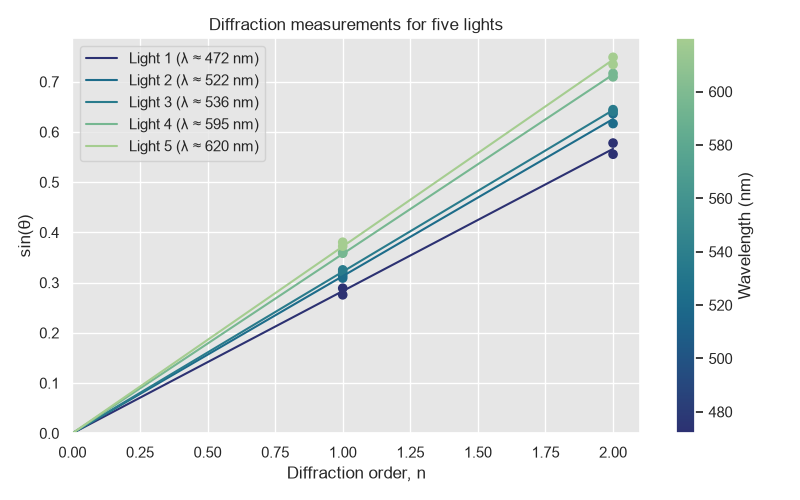
\includegraphics[width=0.8\textwidth]{images/slits_plot.png}
    \caption{Diffraction Measurements for Five Lights}
    \label{fig:slits}
\end{figure}

\subsection{Determination of Planck's Constant and the Work Function}

The maximum kinetic energy of the emitted photoelectrons was determined from the measured stopping potential using

\begin{equation}
    K_{\max}=eV_{\max},
\end{equation}

where \(e=1.602\times10^{-19}\,\mathrm{C}\) is the elementary charge. The resulting energies were plotted against the corresponding LED frequencies, as shown in Figure~\ref{fig:stopping_voltage}.

Einstein's photoelectric equation predicts a linear relationship between kinetic energy and frequency:

\begin{equation}
    K_{\max}=hf-\phi,
\end{equation}

where \(h\) is Planck's constant and \(\phi\) is the work function of the cathode. Comparing this equation with \(y=mx+b\), the gradient of the graph corresponds to Planck's constant, while the vertical intercept is equal to the negative work function.

Using \(K_{\max}=eV_{\max}\) and \(f=c/\lambda\), a linear fit to all five experimental data points tested the energy--frequency dependence predicted by Einstein's equation \cite{einstein1905,millikan1916} and gave

\begin{equation}
    K_{\max} =
    (6.3503\times10^{-34})f
    - 2.7941\times10^{-19},
\end{equation}

where the energy is expressed in joules and the frequency in hertz. The gradient therefore gave the experimental value

\begin{equation}
    h_{\mathrm{exp}} = (6.4\pm0.4)\times10^{-34}\,\mathrm{J\,s}.
\end{equation}

Using the accepted value \(6.626\times10^{-34}\,\mathrm{J\,s}\), the percentage difference is

\begin{equation}
    \frac{|6.350-6.626|}{6.626}\times100\%
    \approx 4.2\%.
\end{equation}

The work function, \(\phi=hf_0\), was obtained from the magnitude of the vertical intercept:

\begin{equation}
    \phi_{\mathrm{exp}}=hf_0 =
    (2.794\pm0.197)\times10^{-19}\,\mathrm{J}.
\end{equation}

Converting this value to electronvolts gives

\begin{equation}
    \phi_{\mathrm{exp}} = (1.7\pm0.1)\,\mathrm{eV}.
\end{equation}

\begin{figure}[H]
    \centering
    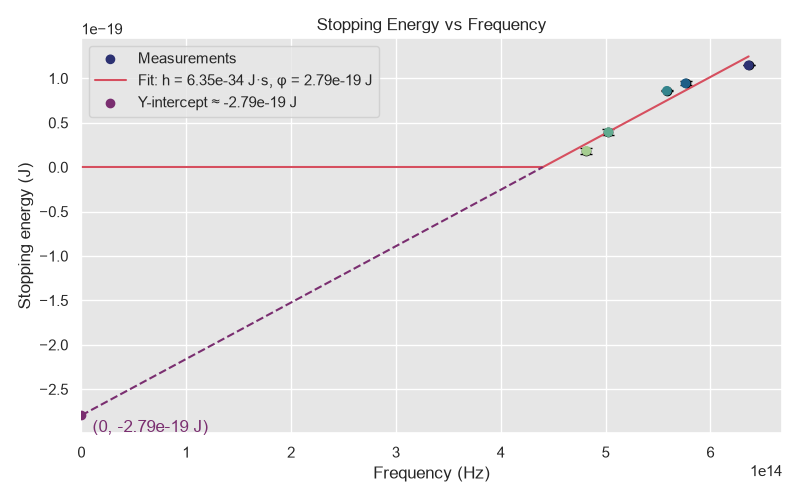
\includegraphics[width=0.8\textwidth]{images/stopping_voltage_plot.png}
    \caption{Stopping Voltage vs Frequency}
    \label{fig:stopping_voltage}
\end{figure}

\subsection{Effect of Light Intensity on the Stopping Potential}

The stopping potential was measured at several intensity settings for four LEDs with wavelengths of approximately \(472\), \(537\), \(522\), and \(597\,\mathrm{nm}\). The measured settings are relative intensity controls, rather than calibrated photon fluxes. The mean stopping potentials are plotted against these settings in Figure~\ref{fig:trends}, and the individual readings are listed in Table~\ref{tab:intensity_data}. For most of the \(472\,\mathrm{nm}\) measurements, \(V_{\max}\) remains near \(0.71\)--\(0.73\,\mathrm{V}\); the \(537\,\mathrm{nm}\) and \(522\,\mathrm{nm}\) series show modestly larger scatter as the setting falls. The \(597\,\mathrm{nm}\) series is especially scattered at its lowest settings, where the measured ranges are very wide. These departures make the low-intensity points less reliable for judging whether the stopping potential is constant.

For visual guidance, each wavelength group was fitted separately with the empirical function
\[
    V_{\max}(I) = \frac{1}{b(I+a)}+c,
\]
where \(I\) is the relative intensity setting. The parameters below are the rounded values reported in the plot legend.

\begin{table}[H]
    \centering
    \begin{tabular}{r r r r}
    \toprule
        Wavelength (nm) & \(a\) & \(b\) & \(c\) (V) \\
    \midrule
        472 & \(-0.04\) & \(890.24\) & \(0.71\) \\
        537 & \(-0.02\) & \(533.16\) & \(0.54\) \\
        522 & \(-0.02\) & \(304.91\) & \(0.59\) \\
        597 & \(-0.05\) & \(156.90\) & \(0.23\) \\
    \bottomrule
    \end{tabular}
    \caption{Rounded parameters of the empirical fits to average stopping potential versus relative intensity. The fit parameters are descriptive and are not physical constants.}
    \label{tab:intensity_fit_parameters}
\end{table}

The parameter \(c\) is the model's limiting value at large \(I\), while \(a\) and \(b\) determine the curvature and horizontal displacement. These fits are empirical rather than a prediction derived from the photoelectric equation: no parameter uncertainties were calculated, and the parameters should not be interpreted as independently measured physical quantities. In particular, the fit for \(597\,\mathrm{nm}\) is strongly affected by the anomalous low-intensity points, so its curve is not a reliable extrapolation. The broad near-constant behaviour at moderate and high settings is qualitatively consistent with the prediction that intensity changes photocurrent, not the maximum photoelectron energy. The data do not establish exact intensity independence, especially at the lowest settings.

\begin{figure}[H]
    \centering
    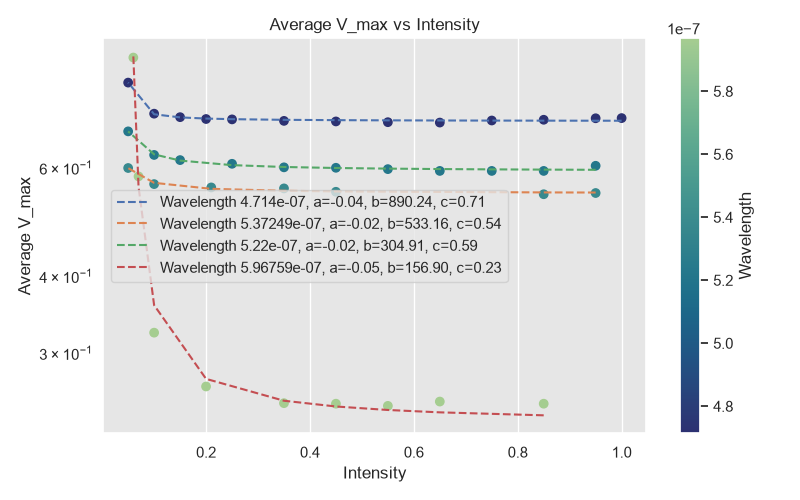
\includegraphics[width=0.8\textwidth]{images/trends_plot.png}
    \caption{Trends of Average $V_{max}$ vs Intensity for Different Wavelengths}
    \label{fig:trends}
\end{figure}

\subsection{Photocurrent--Voltage Fit}

Figure~\ref{fig:photocurrent_iv} shows the measured current as a function of electrode voltage together with a four-parameter sigmoid fit:

\begin{equation}
    I(V) = I_{\mathrm{low}} +
    \frac{I_{\mathrm{sat}}-I_{\mathrm{low}}}
    {1+\exp\!\left[-(V-V_{\mathrm{mid}})/s\right]}.
    \label{eq:iv_sigmoid}
\end{equation}

An unweighted nonlinear least-squares fit to the 44 measurements gives

\begin{align}
    I_{\mathrm{low}} &= (-0.2969 \pm 0.0042)\,\mathrm{nA}, \\
    I_{\mathrm{sat}} &= (3.741 \pm 0.076)\,\mathrm{nA}, \\
    V_{\mathrm{mid}} &= (-0.0160 \pm 0.0085)\,\mathrm{V}, \\
    s &= (0.2320 \pm 0.0029)\,\mathrm{V}.
\end{align}

The fitted curve has \(R^2=0.99989\) and a root-mean-square residual of \(0.0086\,\mathrm{nA}\). Its formal zero-current crossing is \(V\approx(-0.604\pm0.002)\,\mathrm{V}\) in the plotted convention, equivalent to \(+0.604\,\mathrm{V}\) in the recorded voltage convention.

\begin{figure}[H]
    \centering
    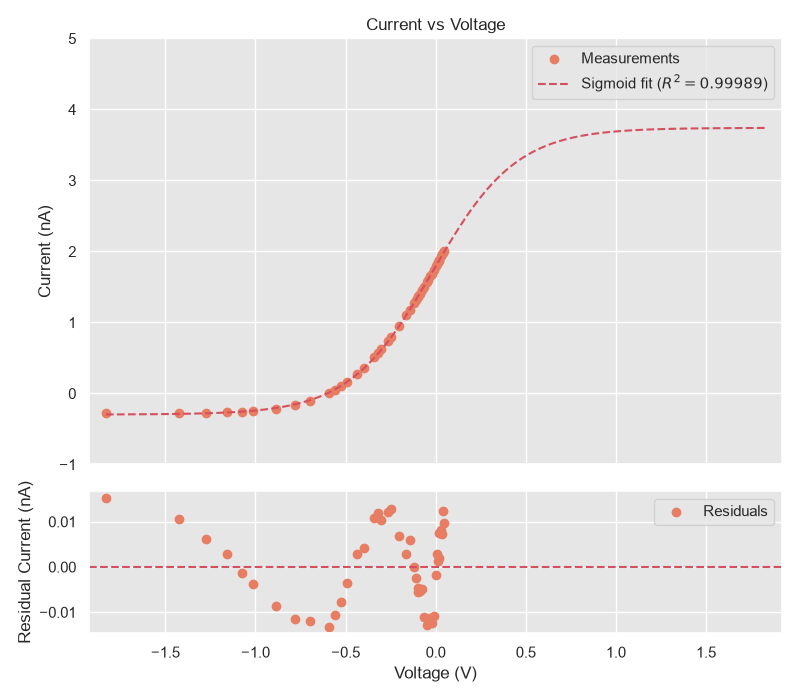
\includegraphics[width=0.8\textwidth]{images/volts_v_amps_plot.png}
    \caption{Measured photocurrent versus electrode voltage and the fitted sigmoid saturation curve.}
    \label{fig:photocurrent_iv}
\end{figure}
\newpage

%================================================
\section{Error Analysis}
%================================================

For each LED, the four diffraction measurements were combined as
\[
    \bar{\lambda}_j =
    \frac{1}{4}\sum_{i=1}^{4}
    \frac{d x_{ij}}{n_{ij}\sqrt{L_j^2+x_{ij}^2}},
    \qquad
    f_j=\frac{c}{\bar{\lambda}_j},
    \qquad
    K_j=eV_j.
\]
The grating spacing \(d\), elementary charge \(e\), and stopping voltages were treated as exact, as specified. The independent position uncertainties were \(\sigma_x=2.0\,\mathrm{mm}\). The distance uncertainty was \(\sigma_L=0.5\,\mathrm{mm}\); it was treated as a shared uncertainty for the five LED groups using the same \(L=0.401\,\mathrm{m}\) setup distance, and as a separate uncertainty for the group using \(L=0.360\,\mathrm{m}\). These nominal distances follow from the tabulated \(x\) and \(\theta\) values.

\begin{table}[H]
    \centering
    \begin{tabular}{c c c c} 
    \hline
    $\lambda$ (nm) & $\sigma_V$ (V) & $\sigma_{eV} $ (eV) & $\sigma_\lambda$ (nm)\\
    \hline
    \color{cyan}472 nm & 0.0005 & $8.0\times10^{-23}$ & 5.59 \\
    \color{JungleGreen}522 nm & 0.001 & $2.3\times10^{-21}$ & 4.42 \\
    \color{Green}536 nm & 0.0145 & $7.2\times10^{-22}$ & 1.37 \\
    \color{YellowOrange}595 nm & 0.0045 & $3.4\times10^{-21}$ & 1.91 \\
    \color{red}620 nm & 0.021 & $3.4\times10^{-21}$ & 4.15 \\
    \hline
    \end{tabular}
    \caption{Stopping-potential repeatability and diffraction-fit wavelength uncertainties for the five LEDs.}
    \label{tab:lambda_uncertainties}
\end{table}

The resulting frequency uncertainties were propagated through the five-point linear fit \(K=hf-\phi\) using first-order covariance propagation. For \(q=(x_1,\ldots,x_{20},L_{0.401},L_{0.360})\), the fitted-parameter covariance is \(C_{h,\phi}=J C_q J^\mathsf{T}\), where \(J\) is the Jacobian of \((h,\phi)\) with respect to the measured positions and setup distances. The separate position and distance contributions are
\[
    \begin{aligned}
    \sigma_{h,\mathrm{geom}} &=
    \sqrt{(16.86\times10^{-36})^2+(0.765\times10^{-36})^2}
    =1.688\times10^{-35}\,\mathrm{J\,s},\\
    \sigma_{\phi,\mathrm{geom}} &=
    \sqrt{(8.990\times10^{-21})^2+(0.166\times10^{-21})^2}
    =8.992\times10^{-21}\,\mathrm{J}.
    \end{aligned}
\]
Thus the geometry-only contribution to the work-function uncertainty is \(\sigma_{\phi,\mathrm{geom}}/e=0.0561\,\mathrm{eV}\). The position contributions above are scaled for \(\sigma_x=2.0\,\mathrm{mm}\); the distance contributions are unchanged.

The wavelength uncertainties in Table~\ref{tab:lambda_uncertainties} are standard errors of the fitted diffraction slopes. For the fit through the origin, the slope standard error is the residual standard deviation divided by \(\sqrt{\sum_i n_i^2}\), using three residual degrees of freedom. Treating this wavelength variation as independent between LEDs, the frequency uncertainties are
\[
    \sigma_{f,j} = \left|\frac{\partial f_j}{\partial\lambda_j}\right|
    \sigma_{\lambda,j}
    = \frac{f_j}{\lambda_j}\sigma_{\lambda,j}.
\]
For the ordinary least-squares slope \(\hat h\), the sensitivity to each fitted frequency is
\[
    \frac{\partial\hat h}{\partial f_j}
    = \frac{(K_j-\bar K)-2\hat h(f_j-\bar f)}
    {\sum_k(f_k-\bar f)^2},
    \qquad
    \sigma_{h,\lambda}^2 =
    \sum_j\left(\frac{\partial\hat h}{\partial f_j}\right)^2
    \sigma_{f,j}^2.
\]
This gives \(\sigma_{h,\lambda}=3.32\times10^{-35}\,\mathrm{J\,s}\). Propagating the same frequency errors through the intercept gives \(\sigma_{\phi,\lambda}=1.75\times10^{-20}\,\mathrm{J}\). Treating these wavelength-fit variations as independent of the position and distance contributions, the combined marginal uncertainties are
\[
    \begin{aligned}
    \sigma_h &= \sqrt{\sigma_{h,\mathrm{geom}}^2+
    \sigma_{h,\lambda}^2}
    = 3.73\times10^{-35}\,\mathrm{J\,s},\\
    \sigma_\phi &= \sqrt{\sigma_{\phi,\mathrm{geom}}^2+
    \sigma_{\phi,\lambda}^2}
    = 1.97\times10^{-20}\,\mathrm{J}
    = 0.123\,\mathrm{eV}.
    \end{aligned}
\]
The combined \(h\) and \(\phi\) uncertainties retain their shared-input covariance. The independence assumption is approximate because both uncertainty estimates originate from the diffraction measurements. Voltage repeatability and instrument calibration are not included in this fit because the voltage readings were treated as exact.

For the photocurrent--voltage sigmoid, the quoted parameter errors are statistical standard errors from an unweighted fit to 44 points. The fit has an RMS residual of \(0.0086\,\mathrm{nA}\); no current-meter or voltage calibration uncertainty is specified, so these errors likewise do not represent the full measurement uncertainty.

\newpage

%================================================
\section{Discussion}

\subsection{Planck's Constant and the Work Function}

The central significance of this experiment is that it tests the energy-transfer relation \(E_\gamma=hf\) proposed in Einstein's 1905 light-quantum theory, rather than merely measuring a material property. The measured stopping potential provides an estimate of the maximum electron energy; a linear increase of \(K_{\max}\) with frequency, with a slope corresponding to \(h\), is the expected signature. Earlier precision work by Millikan quantitatively tested this relation \cite{einstein1905,millikan1916}. Here, the fitted value \(6.350\times10^{-34}\,\mathrm{J\,s}\) is 4.2\% below the accepted value \cite{nistconstants}. The combined propagated uncertainty is \(3.73\times10^{-35}\,\mathrm{J\,s}\), including diffraction-fit variation and the stated position and distance errors. The voltage readings were treated as exact, so this is not a complete experimental uncertainty budget. The result is evidence in support of Einstein's model, not proof from this data set alone.

The fitted work function is \(\phi=hf_0=(1.7\pm0.1)\,\mathrm{eV}\), below the commonly tabulated value of approximately \(2.1\,\mathrm{eV}\) for clean caesium \cite{cesiumworkfunction}. This quoted uncertainty includes diffraction-fit variation and propagated position and distance errors, but not voltage uncertainty. A photocathode's effective work function can differ from that of a clean caesium surface because it depends on surface condition and composition \cite{cesiumworkfunction}. The work-function estimate is particularly sensitive to the fitted intercept.

The measured value lies about \(0.36\,\mathrm{eV}\) below the clean-caesium value, roughly three times the combined uncertainty, so the difference is unlikely to be explained by the propagated errors alone. One possible explanation is degradation or contamination of the caesium photocathode. Caesium is highly reactive, and ageing of the photocell, residual gas in the tube, or oxidation could leave a surface layer whose composition differs from clean caesium and therefore changes the effective work function. This is a hypothesis rather than a conclusion: no independent test of the cathode surface was made, and the direction of the shift depends on the specific surface layer. Other effects could produce a similar offset in the intercept. These include a contact potential difference between the cathode and anode, which shifts the measured stopping potential by a frequency-independent amount, and a systematic bias in identifying the stopping potential from the current--voltage curve (for example from the uncorrected current offset discussed below). Because such offsets change the intercept but not the gradient, they would reduce the extracted work function without necessarily affecting \(h\). Measuring the stopping potential at additional wavelengths, repeating the measurement on a fresh or re-conditioned cathode, and correcting the dark-current baseline would help distinguish these explanations.

\subsection{Intensity Dependence of the Stopping Potential}

The intensity measurements are mostly compatible with the prediction that, at fixed frequency, the stopping potential does not vary systematically with intensity \cite{einstein1905,lenard1902}. The \(471\,\mathrm{nm}\) results remain near \(0.71\)--\(0.73\,\mathrm{V}\) for most settings, and the \(537\,\mathrm{nm}\) readings stay near \(0.54\)--\(0.56\,\mathrm{V}\) except for increased spread at low intensity. In contrast, the two \(597\,\mathrm{nm}\) results at intensities \(0.07\) and \(0.06\) are far above the other readings for that LED. The broad pattern agrees with the idea that frequency determines the maximum energy while intensity mainly changes the number of emitted electrons, but the low-intensity scatter, especially for \(597\,\mathrm{nm}\), prevents a strong quantitative test. The anomalous readings should be checked against the original record rather than excluded without evidence.

Figure~\ref{fig:trends} is also relevant to the historical interpretation. A classical wave picture predicts that increasing the intensity increases the energy delivered to each electron, so \(V_{\max}\) should rise with intensity. The fitted curves instead show that, for most LEDs, \(V_{\max}\) is approximately flat over the intensity range, so the measurements are inconsistent with this classical expectation. This is the same intensity independence that Lenard reported \cite{lenard1902}, and it is what Einstein's model explains \cite{einstein1905}. Strictly, these data do not disprove Lenard's own interpretation, since his observations are consistent with the result here. They contradict only the classical intensity-dependent prediction, and the anomalous low-intensity points limit how firmly even that conclusion can be drawn. Distinguishing Einstein's model from alternatives that also give intensity-independent energies requires the frequency dependence of the stopping potential, which is the linear \(K_{\max}\)--\(f\) relation tested above.

\subsubsection{Why the apparent stopping potential rises at low intensity}

In the ideal Einstein picture each absorbed photon gives a maximum electron energy \(K_{\max}=hf-\phi\), so \(eV_s=hf-\phi\) is independent of intensity; intensity only sets the number of photons per second and therefore the photocurrent. An apparent increase of \(V_s\) at low intensity is therefore not a property of the photoelectric effect itself and is better explained by how the stopping potential is read from the curve. The measured current is \(I(V)=I_{\mathrm{photo}}(V)+I_{\mathrm{off}}\), where \(I_{\mathrm{off}}\) collects the dark current, leakage and electrometer offset, none of which depend on the LED intensity. The zero crossing is displaced from the true photocurrent zero by
\[
\Delta V\approx\frac{I_{\mathrm{off}}}{\mathrm{d}I/\mathrm{d}V}.
\]
Near cutoff the slope \(\mathrm{d}I/\mathrm{d}V\) scales with the photoelectron flux, and hence with the intensity \(\Phi\), so \(\Delta V\propto I_{\mathrm{off}}/\Phi\). The offset is fixed while the signal shrinks, so the displacement of the apparent stopping potential grows as the intensity falls, giving an inverse dependence on intensity. It is largest for the dimmest settings and for the LEDs with the smallest photocurrent, which is where the anomalous \(597\,\mathrm{nm}\) readings occur. A second effect is that, at very low intensity, the few fastest electrons produce a current below the instrument resolution, which would bias the reading in the opposite direction, so the sign of the net shift depends on which effect dominates. Because no dark-current record was taken, this explanation is consistent with the data but could not be tested, and it should be treated as a likely cause rather than a demonstrated one.

\subsection{Photocurrent--Voltage Characteristic}

In the plotted sign convention, the photocurrent--voltage measurements rise from negative current at the most retarding voltages and level off toward positive collecting voltages. The sigmoid describes this measured shape well (\(R^2=0.99989\)); its fitted lower asymptote is \(-0.297\,\mathrm{nA}\), while the fitted saturation current of \(3.741\,\mathrm{nA}\) is an extrapolation beyond the measured voltage range. The measured zero crossing is near \(-0.593\,\mathrm{V}\) in the plot, equivalent to \(+0.593\,\mathrm{V}\) in the table's recorded convention; the fit gives \(-0.604\,\mathrm{V}\), or \(+0.604\,\mathrm{V}\) recorded. The crossing therefore has the expected sign in the plotted convention, but a current baseline or voltage-reference offset remains plausible and no dark-current or zero-offset correction is reported. Consequently, the crossing should not be treated as a definitive physical stopping-potential measurement, and the sigmoid fit is not used to calculate Planck's constant or the work function.

No dark-current measurement (current with the LED covered or switched off) was recorded, so the dark offset could not be subtracted. Its effect can still be bounded: a constant offset \(I_\mathrm{dark}\) shifts the apparent zero crossing by approximately \(\Delta V \approx I_\mathrm{dark}/(\mathrm{d}I/\mathrm{d}V)\), evaluated at the crossing. This shift is largest for the dimmest LEDs, where the photocurrent and the slope are smallest. A shift common to all LEDs changes the intercept (and hence \(\phi\)) but not the gradient, whereas an offset that varies between LEDs would also bias \(h\). It is therefore treated here as an unquantified systematic error rather than included in the propagated uncertainty. Recording a dark curve at each voltage and subtracting it before locating the zero crossing would remove this.

\subsubsection{Origin of the sigmoid shape}

At large collecting voltages every emitted electron reaches the anode, so the current saturates at \(I_s\propto\Phi\), the photon flux multiplied by the quantum efficiency. Under a retarding voltage \(V\), only electrons with kinetic energy \(K\ge e|V|\) reach the anode. If \(N(K)\) is the energy distribution of the emitted electrons, then
\[
I(V)\propto\int_{e|V|}^{K_{\max}}N(K)\,\mathrm{d}K,
\]
so the measured current is the cumulative distribution of the photoelectron energies. This distribution is a broad peak between \(0\) and \(K_{\max}\) rather than a single value: electrons originate from different states below the Fermi level and from different depths, and lose varying amounts of energy by scattering before escaping the surface. The derivative \(\mathrm{d}I/\mathrm{d}V\propto N(K)\) is therefore bell-shaped, and its integral is flat at both ends and steepest in the middle, which is a sigmoid. Near cutoff the current falls smoothly to zero rather than sharply, further softened by thermal broadening of the Fermi edge and non-uniform fields between the electrodes. A small negative lower asymptote, such as the fitted \(-0.297\,\mathrm{nA}\), is consistent with a reverse current from stray light liberating electrons at the anode together with leakage, and is not a property of the cathode.

This has a consequence for the stopping potential. Because the curve has no sharp edge, the true \(V_s\), at which the \(K_{\max}\) electrons are just stopped, lies at the foot of the curve, whereas the zero crossing lies above it. The resulting bias is similar for all LEDs and therefore mainly affects the intercept (\(\phi\)) rather than the gradient (\(h\)), consistent with the offset discussion above.

\subsection{Limitations}

The main limitations are the five-point linear fit, the omission of voltage repeatability and calibration uncertainty from the propagated errors, and scattered low-intensity results. Improving the diffraction-position and distance measurements, repeating stopping-potential measurements at each wavelength, including voltage uncertainties, and measuring/correcting the dark-current baseline would provide a more complete uncertainty budget and a more reliable comparison with theory.

\newpage

%================================================
\section{Conclusion}

The photoelectric effect was used to estimate Planck's constant and the effective work function of the caesium-coated photocathode. The fitted values were \(h=(6.4\pm0.4)\times10^{-34}\,\mathrm{J\,s}\) and \(\phi=(1.7\pm0.1)\,\mathrm{eV}\); the Planck-constant estimate is 4.2\% below the accepted value \cite{nistconstants}. These uncertainties include diffraction-fit variation and propagated diffraction-position and distance errors, but treat the stopping voltages as exact and therefore do not represent the full experimental uncertainty. The linear energy--frequency relation tested here is the distinctive prediction of Einstein's 1905 light-quantum account and underlies subsequent precision determinations of \(h\) from the photoelectric effect \cite{einstein1905,millikan1916}. The result is historically and physically significant as a laboratory-scale test of quantised light energy, but it should not be presented as definitive proof. The low-intensity data include conspicuous anomalies. The intensity series generally showed little change in stopping potential, while the current--voltage curve exhibited a saturating rise. Once the plot's sign convention is accounted for, its zero crossing has the expected sign, but the uncorrected current baseline prevents it from serving as an independent stopping-potential measurement.
%================================================

\newpage

%================================================
\section{References}
\printbibliography[heading=none]
%================================================

\newpage

%================================================
\appendix
\section{Appendix}
\subsection{Diffraction Data}

\begin{table}[H]
    \centering
    \begin{tabular}{lllll}
    \hline
        n & x & theta & sin theta & lambda \\ \hline
        1 & 0.115 & 0.279287476 & 0.275670803 & 4.59451E-07 \\ 
        1 & 0.121 & 0.293057525 & 0.288880738 & 4.81468E-07 \\ 
        2 & 0.268 & 0.589152689 & 0.555656758 & 4.63047E-07 \\ 
        2 & 0.284 & 0.616227743 & 0.577960875 & 4.81634E-07 \\ 
        1 & 0.136 & 0.326978289 & 0.321182887 & 5.35305E-07 \\ 
        1 & 0.138 & 0.331444509 & 0.325409256 & 5.42349E-07 \\ 
        2 & 0.335 & 0.695963465 & 0.641125135 & 5.34271E-07 \\ 
        2 & 0.338 & 0.700353452 & 0.644487982 & 5.37073E-07 \\ 
        1 & 0.154 & 0.366672413 & 0.358511035 & 5.97518E-07 \\ 
        1 & 0.155 & 0.368843839 & 0.36053727 & 6.00895E-07 \\ 
        2 & 0.404 & 0.789124854 & 0.709737033 & 5.91448E-07 \\ 
        2 & 0.412 & 0.798927473 & 0.716608442 & 5.97174E-07 \\ 
        1 & 0.161 & 0.38179559 & 0.372587371 & 6.20979E-07 \\ 
        2 & 0.434 & 0.824898565 & 0.734478949 & 6.12066E-07 \\ 
        1 & 0.165 & 0.390356166 & 0.380517812 & 6.34196E-07 \\ 
        2 & 0.453 & 0.846213009 & 0.748775673 & 6.2398E-07 \\ \hline
    \end{tabular}
    \caption{Measured values of diffraction order, position, angle, and wavelength.}
    \label{tab:diffraction_data}
\end{table}

\subsection{Stopping Voltage Data}
\begin{table}[H]
    \centering
    \begin{tabular}{llll}
    \hline
        Frequency ($\mathrm{Hz}$) & $V_\text{max,min}$ ($\mathrm{V}$) & $V_\text{max,max}$ ($\mathrm{V}$) & $K_{\max}$ ($\mathrm{J}$) \\ \hline
        6.36402E+14 & 0.715 & 0.716 & 1.14623E-19 \\ 
        5.76248E+14 & 0.588 & 0.590 & 9.43684E-20 \\
        5.584E+14 & 0.532 & 0.541 & 8.59473E-20 \\ 
        5.02716E+14 & 0.225 & 0.267 & 3.94092E-20 \\
        4.81692E+14 & 0.1 & 0.129 & 1.83429E-20 \\ \hline
    \end{tabular}
    \caption{Measured frequency, stopping-potential range, and corresponding maximum kinetic energy.}
    \label{tab:stopping_voltage_data}
\end{table}

\subsection{Intensity Data}
\begin{table}[H]
    \centering
    \begin{tabular}{lllll}
    \hline
        Intensity & $V_\text{max,min}$ & $V_\text{max,max}$ & $ V_\text{max,avg}$ & wavelength ($\lambda$) \\ \hline
        1 & 0.721 & 0.723 & 0.722 & 4.714E-07 \\ 
        0.95 & 0.721 & 0.722 & 0.7215 & 4.714E-07 \\ 
        0.85 & 0.717 & 0.718 & 0.7175 & 4.714E-07 \\ 
        0.75 & 0.715 & 0.716 & 0.7155 & 4.714E-07 \\ 
        0.65 & 0.709 & 0.711 & 0.71 & 4.714E-07 \\ 
        0.55 & 0.71 & 0.712 & 0.711 & 4.714E-07 \\ 
        0.45 & 0.712 & 0.714 & 0.713 & 4.714E-07 \\ 
        0.35 & 0.713 & 0.716 & 0.7145 & 4.714E-07 \\ 
        0.25 & 0.717 & 0.72 & 0.7185 & 4.714E-07 \\ 
        0.2 & 0.718 & 0.721 & 0.7195 & 4.714E-07 \\ 
        0.15 & 0.723 & 0.726 & 0.7245 & 4.714E-07 \\ 
        0.1 & 0.731 & 0.737 & 0.734 & 4.714E-07 \\ 
        0.05 & 0.818 & 0.831 & 0.8245 & 4.714E-07 \\ \hline
        0.95 & 0.543 & 0.548 & 0.5455 & 5.37249E-07 \\ 
        0.85 & 0.539 & 0.547 & 0.543 & 5.37249E-07 \\ 
        0.45 & 0.541 & 0.555 & 0.548 & 5.37249E-07 \\ 
        0.35 & 0.549 & 0.561 & 0.555 & 5.37249E-07 \\ 
        0.21 & 0.545 & 0.569 & 0.557 & 5.37249E-07 \\ 
        0.1 & 0.541 & 0.587 & 0.564 & 5.37249E-07 \\ 
        0.05 & 0.528 & 0.67 & 0.599 & 5.37249E-07 \\ \hline
        0.85 & 0.23 & 0.266 & 0.248 & 5.96759E-07 \\ 
        0.65 & 0.229 & 0.271 & 0.25 & 5.96759E-07 \\ 
        0.55 & 0.223 & 0.269 & 0.246 & 5.96759E-07 \\ 
        0.45 & 0.219 & 0.277 & 0.248 & 5.96759E-07 \\ 
        0.35 & 0.217 & 0.28 & 0.2485 & 5.96759E-07 \\ 
        0.2 & 0.203 & 0.326 & 0.2645 & 5.96759E-07 \\ 
        0.1 & 0.181 & 0.466 & 0.3235 & 5.96759E-07 \\ 
        0.07 & 1.005 & 0.156 & 0.5805 & 5.96759E-07 \\ 
        0.06 & 0.137 & 1.674 & 0.9055 & 5.96759E-07 \\ \hline
    \end{tabular}
    \caption{Measured values of intensity, maximum voltage, average maximum voltage, and wavelength for different light intensities.}
    \label{tab:intensity_data}
\end{table}

\subsection{Voltage and Current Data}
\begin{table}[H]
    \centering
    \begin{tabular}{ll}
    \hline
        Voltage ($\mathrm{V}$) & Current ($\mathrm{nA}$) \\ \hline
        0.046 & 2 \\ 
        0.04 & 1.977 \\ 
        0.037 & 1.959 \\ 
        0.031 & 1.934 \\ 
        0.02 & 1.886 \\ 
        0.016 & 1.863 \\ 
        0.012 & 1.845 \\ 
        0.007 & 1.825 \\ 
        0 & 1.79 \\ 
        -0.011 & 1.733 \\ 
        -0.021 & 1.688 \\ 
        -0.03 & 1.65 \\ 
        $\vdots $ & $\vdots $ \\
        -0.398 & 0.36 \\ 
        -0.439 & 0.2677 \\ 
        -0.49 & 0.163 \\ 
        -0.524 & 0.102 \\ 
        -0.557 & 0.05 \\ 
        -0.593 & 0 \\ 
        -0.698 & -0.106 \\ 
        -0.782 & -0.165 \\ 
        -0.884 & -0.212 \\ 
        -1.011 & -0.246 \\ 
        -1.077 & -0.257 \\ 
        -1.16 & -0.265 \\ 
        -1.274 & -0.273 \\ 
        -1.425 & -0.277 \\ 
        -1.83 & -0.28 \\ \hline
    \end{tabular}
    \caption{Measured values of voltage and current for the photoelectric effect experiment.}
    \label{tab:volts_v_amps}
\end{table}


\end{document}